\documentclass[sigconf,review,anonymous, table]{acmart}
%\documentclass[sigconf,anonymous, table]{acmart}
%\documentclass[manuscript,screen, table]{acmart}
\usepackage{paralist}
\usepackage{enumitem,kantlipsum}
\usepackage{pgf-pie}
\usepackage{tikz}
\usepackage[most]{tcolorbox}
\usepackage{etoolbox}
\usepackage{fp}
\usepackage{subcaption}
\usepackage{mwe}
\usepackage{xspace}
\usepackage{eurosym}
\usepackage{mdframed,ifthen}
\usepackage{array}
\tcbuselibrary{listings,breakable}
\usepackage{placeins}

\def\bf{\textbf}
\def\eq {Equation~}
\def\eqm {Eq~}
\def\eqs {Equations~}
\def\fig {Figure~}
\def\figs {Figures~}
\def\tbl {Table~}
\def\tbls {Tables~}
\def\ie{\textit{i.e.,}}
\def\eg{\textit{e.g.,}}
\def\sec {Section~}
\def\secs {Sections~}
\def\alg {Algorithm~}
\def\algs {Algorithms~}
\def\app {Appendix~}
\def\it{\textit}
\def\tr{\textrm}
\def\tt{\mct}
%\newcommand{\ib}[1]{{\textbf {\textit { #1}}}}
%\newcommand{\ts}[1]{{\textsc {{ #1}}}}
\newcommand{\mct}[1]{{\footnotesize {\texttt {#1}}}}

\newcommand{\qu}[1]{{\it{``#1''}}}
\newcommand{\api}[1]{{\sf{\texttt\small{#1}}}}
\newcommand{\callout}[1]{{\vspace{1mm}\noindent{\fbox{\parbox{0.97\columnwidth}{#1}}}\vspace{1mm}}}
\usepackage{paralist}
\usepackage{hyperref}
\usepackage{soul}

\normalsize
\let\labelindent\relax
\usepackage{enumitem}

%% We use a different version in main and appendix! In main we allow
%% breaking, in appendix we do not.
\newenvironment{practice}[2]
    {
   \begin{center}\begin{tcolorbox}[width=.48\textwidth, skin=enhanced jigsaw, arc=0pt, title={\textbf{Guiding Principle #1: #2}}]
    
    }
    {\end{tcolorbox}\end{center} }

\newcommand{\nd}{\vspace{1mm}\noindent}
\usepackage{caption}
%\usepackage[toc,page]{appendix}
\usepackage{tikz}
\newcommand*\circled[1]{\tikz[baseline=(char.base)]{
            \node[shape=circle,draw,inner sep=1pt] (char) {#1};}}

 \lstset{
         language=Java,
         basicstyle=\scriptsize\ttfamily, % Standardschrift
         %numbers=left,               % Ort der Zeilennummern
         numberstyle=\tiny,          % Stil der Zeilennummern
         %stepnumber=2,               % Abstand zwischen den Zeilennummern
         numbersep=5pt,              % Abstand der Nummern zum Text
         tabsize=2,                  % Groesse von Tabs
        % extendedchars=true,         %
         breaklines=true,            % Zeilen werden Umgebrochen
%         keywordstyle=\color{black},
 %   	 frame=single,
 %        keywordstyle=[1]\textbf,    % Stil der Keywords
 %        keywordstyle=[2]\textbf,    %
 %        keywordstyle=[3]\textbf,    %
 %        keywordstyle=[4]\textbf,   \sqrt{\sqrt{}} %
         stringstyle=\color{white}\ttfamily, % Farbe der String
         showspaces=false,           % Leerzeichen anzeigen ?
         showtabs=false,             % Tabs anzeigen ?
         xleftmargin=17pt,
         framexleftmargin=17pt,
         framexrightmargin=5pt,
         framexbottommargin=4pt,
         %backgroundcolor=\color{lightgray},
         showstringspaces=false,      % Leerzeichen in Strings anzeigen ?
     %    escapeinside={\%*}{*)}
 }
\usepackage{rotating}
\usepackage{pdflscape}
\lstdefinestyle{inlinecode}{basicstyle={\ttfamily\scriptsize\bfseries}}
%\newcommand\code{\lstinline[style=inlinecode]}
%\newcommand{\urls}[1]{{\scriptsize\url{#1}}}
\usepackage{tcolorbox}
\newcommand{\emt}[1]{\emph{``#1''}}
\usepackage{paralist}
\usepackage[outercaption]{sidecap}    
%\usepackage{unicode-math}
\usepackage{amssymb}% http://ctan.org/pkg/amssymb
\usepackage{pifont}% http://ctan.org/pkg/pifont
\newcommand{\cmark}{\ding{51}}%
\newcommand{\xmark}{\ding{55}}%

\newcommand{\dc}[1]{\href{https://devrant.com/rants/#1/}{$R_{#1}$}}

\usepackage{enumitem}
\hypersetup{
    colorlinks=true,
    linkcolor=blue,
    filecolor=magenta,      
    urlcolor=cyan,
}
\newtcolorbox
{mybox}[2][]{colbacktitle=red!10!white,
colback=blue!10!white,coltitle=black!70!black,
title={#2},fonttitle=\bfseries,#1}

\usepackage{xcolor}
\definecolor{ao(english)}{rgb}{0.0, 0.5, 0.0}
\newcommand{\mybars}[3]{
  {\color{red}\rule{#1pt}{6pt}}
  {\color{yellow}\rule{#2pt}{6pt}}
  {\color{ao(english)}\rule{#3pt}{6pt}}
}
\newcommand{\mybarsbwv}[3]{
  {#1\%\color{black!90}\rule{#1pt}{6pt}}
  {#2\%\color{black!50}\rule{#2pt}{6pt}}
  {#3\%\color{black!20}\rule{#3pt}{6pt}}
}
\newcommand{\mybarsbw}[3]{
  {\color{black!90}\rule{#1pt}{6pt}}
  {\color{black!50}\rule{#2pt}{6pt}}
  {\color{black!20}\rule{#3pt}{6pt}}
}
\newcommand{\mybarsbwa}[3]{
  {#1\%Negative~\color{black!90}\rule{#1pt}{6pt}}\\
  {#2\%Neutral~\color{black!50}\rule{#2pt}{6pt}}\\
  {#3\%Positive~\color{black!20}\rule{#3pt}{6pt}}
}

%\newcommand{\rev}[1]{\textcolor{blue}{ #1}}
\newcommand{\rev}[1]{#1}
\newcommand{\newrev}[1]{\textcolor{blue}{ #1}}
\newcommand{\as}[1]{{\textcolor{magenta}{\sf{\texttt\small{#1}}}}}

\newcommand{\code}[1]{\textsc{#1}\normalfont}
\newcommand{\ab}[1]{{\color{red}{Ann: #1}}}
\newcommand{\numInterviews}{24\xspace}
\newcommand{\todo}[1]{{\color{red}{\textbf{#1}}}}

 %% Ann: I hate the way \qw looks so I've replaced \qw with this new command, \qqw. If the consensus is to return to the look of \qw, this command can be redefined.
 \newcommand{\qqw}[2]{{\textbf{#2}} (#1)\xspace} %% Usage: \qqw{F}{stability}
 \newcommand{\qww}[1]{(#1)\xspace} %% Usage: \qww{F}



\newcommand{\gias}[1]{\textcolor{red}{{[Gias: #1]}}}

% Used to format quotations. Usage:
% Attributed quote: \quotebox{P4}{That's annoying.}
% Unattributed quote: \quotebox{}{I've heard the comment.}
\newenvironment{smallquote}%
{\list{}{\leftmargin=0.15in\rightmargin=0.15in}\item[]}%
  {\endlist}
\newcommand{\quotebox}[2]{\begin{smallquote}\textit{``#2''}\ifthenelse{\equal{#1}{}}{}{ \mbox{-}~#1}\end{smallquote}}

\newenvironment{observation}[2]{
        \begin{mdframed}[
                frametitle={\colorbox{white}{\space #1}},
                innertopmargin=0pt,
                frametitleaboveskip=-\ht\strutbox,
                frametitlealignment=\raggedright,
                nobreak=true,
                skipabove=10pt,
                skipbelow=10pt,
        ]%
        \label{#2}}{\end{mdframed}}



\newcounter{recommendation}[section]
\renewcommand{\therecommendation}{\arabic{recommendation}}

\newenvironment{recommendation}[1]{
        %\refstepcounter{observation}
        \addtocounter{recommendation}{1}
        \begin{mdframed}[
                frametitle={\colorbox{white}{\space Recommendation \therecommendation\space}},
                innertopmargin=0pt,
                frametitleaboveskip=-\ht\strutbox,
                frametitlealignment=\raggedright,
                nobreak=true,
                skipabove=10pt,
                skipbelow=10pt,
        ]%
        \label{#1}}{\end{mdframed}}


\def\nonzero#1#2{%
    \ifnum #1 > 0
      #1#2
    \fi
}


% \newcommand{\horizontalbars}[4]{
% {{\color{black}\rule{#1pt}{4pt}}  \nonzero{#1}{C}}
% {{\color{black!50}\rule{#2pt}{4pt}}  \nonzero{#2}{F}}
% {{\color{black!20}\rule{#3pt}{4pt}}  \nonzero{#3}{P}}
% {{\color{black!40}\rule{#4pt}{4pt}} \nonzero{#4}{S}}

% }

% \newcommand{\horizontalbars}[5]{
% {{\color{black}\rule{#1pt}{4pt}}  \nonzero{#1}{NA}}
% {{\color{red}\rule{#2pt}{4pt}}  \nonzero{#2}{AS}}
% {{\color{green}\rule{#3pt}{4pt}}  \nonzero{#3}{EU}}
% {{\color{blue}\rule{#4pt}{4pt}} \nonzero{#4}{AU}}
% {{\color{black!50}\rule{#5pt}{4pt}} \nonzero{#5}{SA}}
% }


\newcommand{\horizontalbars}[5]{
{{\color{black}\rule{\fpeval{5*(#1)}pt}{4pt}}\nonzero{#1}{}}{{\color{red}\rule{\fpeval{5*(#2)}pt}{4pt}}\nonzero{#2}{}}{{\color{green}\rule{\fpeval{5*(#3)}pt}{4pt}}\nonzero{#3}{}}{{\color{blue}\rule{\fpeval{5*(#4)}pt}{4pt}}\nonzero{#4}{}}{{\color{black!50}\rule{\fpeval{5*(#5)}pt}{4pt}}\nonzero{#5}{}}
}

%\newcommand{\mybarsbwa}[4]{}
% \\   {C\color{black!90}\rule{#1pt}{6pt}}#1 {P\color{black!70}\rule{#2pt}{6pt}}#2 {F\color{black!40}\rule{#3pt}{6pt}}#3 {S\color{black!20}\rule{#4pt}{6pt}}#4
% }


%\newcommand{\qq}[2]{} % remove all quotes
%\newcommand{\qq}[2]{\textit{"#1"}$_{#2}$} % inline quotes
%\newcommand{\qi}[2]{\textit{"#1"}$_{#2}$} % inline quotes
%\newcommand{\qq}[2]{\begin{quote}"#1"$_{#2}$\end{quote}} % stylized quotes

\newcommand{\qi}[2]{\quotebox{#2}{#1}}
\newcommand{\qq}[2]{\quotebox{#2}{#1}} 
\newcommand{\qqi}[2]{\textit{"#1"} - {#2}} % inline quotes




%This is an apple {\def\svgwidth{2cm}\input{name.pdf_tex}} and more text
%https://tex.stackexchange.com/questions/374192/how-to-use-figures-as-inline-images
%https://tex.stackexchange.com/questions/313927/tikz-picture-inline
%https://tex.stackexchange.com/questions/7032/good-way-to-make-textcircled-numbers
\newcommand{\qw}[2]{\textbf{#2}\tikz[baseline=(char.base)]{
    \node[shape=circle,fill=blue!20,inner sep=.5pt] (char){#1};}}

\newcommand{\tc}[0]{\textcolor{green}{ [add citation]}}

% following command is used to highlight text/numbers which can be changed after all the inerview/data collection is done. 
\newcommand{\td}[1]{\textcolor{blue}{(#1)}}

\newcommand{\autourfill}[1]{\tikz[baseline=(X.base)]\node [draw=blue,fill=blue!40,semithick,rectangle,inner sep=2pt, rounded corners=3pt] (X) {#1};}

\newcommand{\autouroutline}[1]{\tikz[baseline=(X.base)]\node [draw=blue,fill=white,semithick,rectangle,inner sep=2pt, rounded corners=3pt] (X) {#1};}

\newcommand{\autourbox}[1]{\tikz[baseline=(X.base)]\node [draw=black!70,fill=white,semithick,rectangle,inner sep=2pt, rounded corners=3pt] (X) {#1};}

\newcommand{\autourhighlight}[1]{\tikz[baseline=(X.base)]\node [draw=none,fill=red!20,semithick,rectangle,inner sep=2pt, rounded corners=3pt](X){#1};}




\newcommand\actor[1]{\textbf{Actor:}  #1\vspace*{.5em}\\} 
\newcommand\condition[1]{\textbf{Condition:}  #1\vspace*{.5em}\\} 
\newcommand\concern[1]{\textbf{Concern:} #1\vspace*{.5em}\\}
\newcommand\solution[1]{\textbf{Solution:} #1\vspace*{.5em}\\ }
\newcommand\consideration[1]{ \textbf{Consideration:} #1 }
\newcommand\steps[1]{\vspace*{.5em}\\\textbf{Steps:} #1}
\newcommand\example[2]{\vspace*{.5em}\\\textbf{Example Data:} \qqi{#1}{#2}}

%\newcommand{minaoar}[1]{\textcolor{blue}{Minaoar: #1}}

%\newcommand\minaoar[1]{\textcolor{blue}{#1}}
\newcommand{\minaoar}[1]{\textcolor{blue}{{[Minaoar]: #1}}}

  \setlength\heavyrulewidth{0.30ex}
  \setlength\cmidrulewidth{0.10ex}
  \setlength\lightrulewidth{0.10ex}
\AtBeginDocument{%
  \providecommand\BibTeX{{%
    \normalfont B\kern-0.5em{\scshape i\kern-0.25em b}\kern-0.8em\TeX}}}

\setcopyright{acmcopyright}
\copyrightyear{2023}
\acmYear{2023}
\acmDOI{XXXXXXX.XXXXXXX}

%% These commands are for a PROCEEDINGS abstract or paper.
\acmConference[ESEC/FSE 2023]{The 31st ACM Joint European Software Engineering Conference and Symposium on the Foundations of Software Engineering}{11 - 17 November, 2023}{San Francisco, USA}

%
%  Uncomment \acmBooktitle if th title of the proceedings is different
%  from ``Proceedings of ...''!
%
%\acmBooktitle{Woodstock '18: ACM Symposium on Neural Gaze Detection,
%  June 03--05, 2018, Woodstock, NY} 
\acmPrice{15.00}
\acmISBN{978-1-4503-XXXX-X/18/06}

\begin{document}

\title{Appendix to Process, Factors, Conditions and Guiding Principles: A Model of Software Library Adoption in Industry}


\author{Minaoar Tanzil}
%\authornote{Both authors contributed equally to this research.}
\email{minaoar.tanzil@ucalgary.ca}
%\orcid{1234-5678-9012}
\author{Gias Uddin}
%\authornotemark[1]
\email{gias.uddin@ucalgary.ca}
\author{Ann Barcomb}
%\authornotemark[1]
\email{ann.barcomb@ucalgary.ca}
\affiliation{%
  \institution{University of Calgary}
  \streetaddress{P.O. Box 1212}
  \city{Calgary}
  \state{Alberta}
  \country{Canada}
  \postcode{T2N 1N4}
}


%%
%% By default, the full list of authors will be used in the page
%% headers. Often, this list is too long, and will overlap
%% other information printed in the page headers. This command allows
%% the author to define a more concise list
%% of authors' names for this purpose.
\renewcommand{\shortauthors}{Tanzil et al.}

\maketitle
\balance
%%%%%%% Appendix
\pagebreak
\section{Methodology}

Figure~\ref{fig:methodology} provides an overview of the overall research method which was applied to the study.

\begin{figure*}
    \centering
    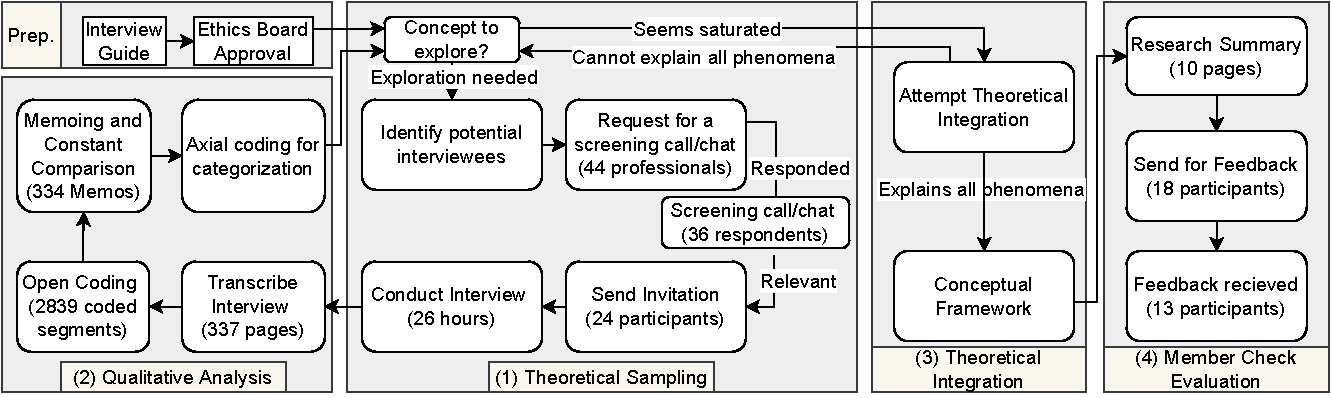
\includegraphics[scale=.75]{images/methodology.pdf}
    \caption{Grounded theory research method applied}
    \label{fig:methodology}
\end{figure*}


\section{Saturation}
\begin{figure*}
    \centering
    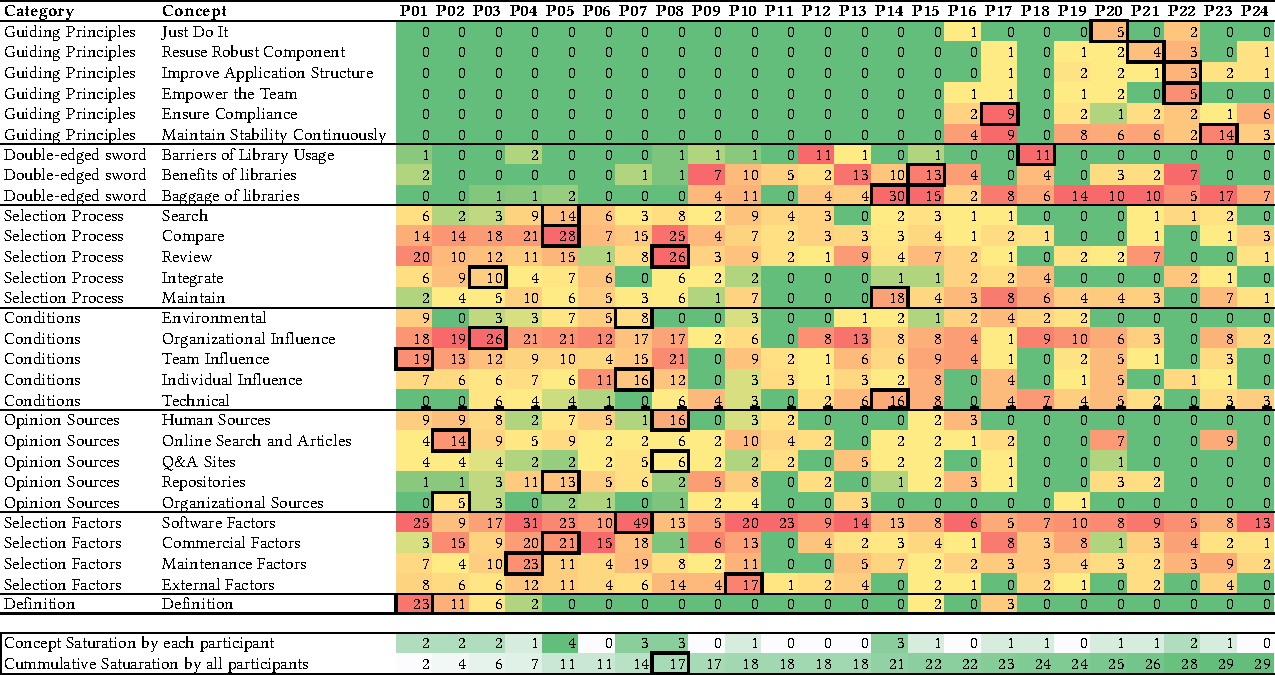
\includegraphics[scale=0.8]{images/saturation.pdf}
    \caption{Heatmap of concept saturation over the interviews. Red refers to higher discussion of a concept by an interviewee, the number refers to how many times interviewee has discussed a concept. Green refers to lower discussion of concepts by an interviewee.}
    \label{fig:saturation}
\end{figure*}
Figure~\ref{fig:saturation} shows how the concepts were discussed during each interview. The number denote how many times a concept was discussed by one particular interview. The more a participant discussed about a particular concept, the more red the corresponding cell is. For example, library search and analysis process was most discussed by P5 and after their interview, subsequently we did not have much to discuss about the search process.  After P8, the concept almost saturated and we discussed very little about this concept with subsequent interviewees.

\begin{table*}[]
    \centering
    \begin{tabular}{p{.4cm}p{4cm}p{6cm}p{6cm}}%{llll}
    \toprule
    P\# & Concept we wanted to enhance & Why we selected this Participant & Concepts they enriched significantly \\ 
    \midrule
P1 & Initial process and factors & Architect of a large system & Library definition, factors, influences \\ 
P2 & Licensing and Security Issues & Working in a large structured company & License, company technology \\ 
P3 & Mobile development Factors & 12+ years experienced in mobile application & Cost, company tech, comparison  \\ 
P4 & Long term maintenance concerns & Being a CEO, takes decisions considering long term impact & Company application domain, active development of library \\ 
P5 & Decision making processes & Stablishing the processes in a startup team & Information search, company culture \\ 
P6 & Open Source factors & Has experience regarding OSS contribution and research & Open source, Personal motivation \\ 
P7 & Factors for a startup & Being a startup CTO may share different priorities & Flexibility, Ease of Installation, Community Support \\ 
P8 & Performance factors & Working in a cloud company that may requiew high performing libraries & Familiarity, Team Discussion, Library Migration \\ 
P9 & Migration scenarios & Experienced to migrate company tech stack as architect & Legal risks, Lack of Stability, Less prefered than native support \\ 
P10 & Visualization and front end libraries & Working as web developer for over a decade & Customer support, flexibility, existing repository \\ 
P11 & Machine learning libraries & Experienced in machine learning in gradudate research studies and in industry & Talk to people, Performance, Outstanding library selection \\ 
P12* & DevOps Process for Library Security Issues & Consulted dozens of companies in DevOps process establishment & Barriers of library usage, Baggage of libraries \\ 
P13 & Selection process in large organizations for legal and security risks & Has been an architect in a large team for 10+ years & Consent Process, Benefits of libraries, Tech Expert Opinion \\ 
P14 & Library migration scenarios & Experienced in managing mobile apps with large user base in all platforms & Make life easy, Life long maintenance, Migration to other library \\ 
P15 & Organizational process and motivation for libraries & Experienced in organization process since increased dev team from 3 to 300 & Delivery Deadline, Don't Reinvent the wheel, Feature criticality \\ 
P16* & Process of security concerns & Cerified security professional actively developing security products & License issues, Data Transfer Security, Geographic Impact  \\ 
P17 & Security Process & Delivers custom software to customers and maintains SecOps in CI/CD & Post Integration Maintenance for Security \\ 
P18 & C++ libraries in large scale long term products & Leads development of a 30 year old product written in C++ with 2M lines of code & Lifelong Maintenance Burden, Compatibility, Uniform Coding Style \\ 
P19 & Company Culture, Open Source, Concept Saturation & Experienced working in start-up and large organizations who open source libraries & Standard practices in large organizations, Considerations in open source \\ 
P20 & Challenges in mobile application libraries, Concept Saturation & Full career in mobile app development, mostly in iOS which requires more maintenance & Lifelong Maintenance Burden, Abandoned Libraries, Migration \\ 
P21 & Company Culture, Open Source, Concept Saturation & Works full-time in a prominent open core company & Company policies, Guiding Principles \\ 
P22 & Guiding Principles, Open Source & Experienced in persuing large corporation for open source library adoption & Guiding Principles \\ 
P23 & ML libraries & Working in South America in ML domain & ML Library Dependency Issues \\ 
P24 & Company Culture, Industry, ML Libraries & Working in health sector using ML libraries extensively. & ML Library deployment and upgrade issues \\ 

\bottomrule
    \end{tabular}
    \caption{How we recruited interview participants following theoretical sampling for Concept Saturation. (We could not enhance targeted concepts from the *-marked participants (P12, P16), rather enriched other important concepts.)}
    \label{tab:theoritcal-sampling}
\end{table*}

%% Ann: this is just an alternate view of our main figure and I don't think it is useful
%\begin{figure}
%    \centering
%    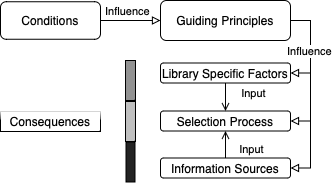
\includegraphics[scale=0.6]{images/Interaction-with-guiding-principles-5.png}
%    \caption{Interaction of guiding principles with the major concepts of software library adoption process}
  %  \label{fig:gp-interaction}
%\end{figure}


\section{Code System}

Figure~\ref{fig:process} shows the relationship between major categories, categories, and concepts in the code system for the major categories steps and source. These concepts and categories contribute to the conceptual framework of the software library adoption process.

\begin{figure*}
    \centering
    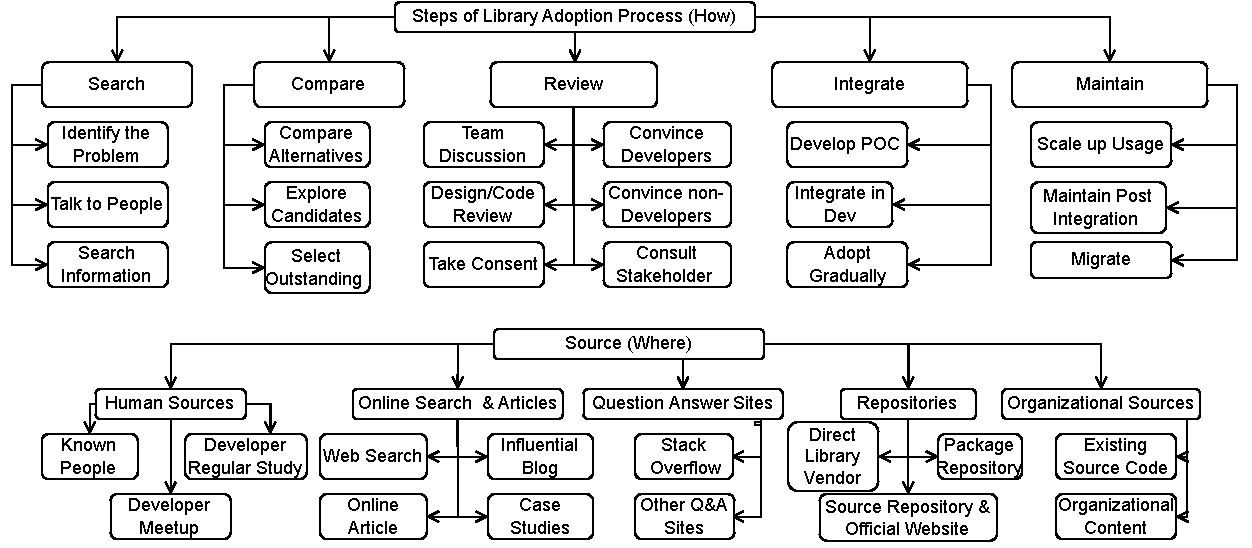
\includegraphics[scale=0.85]{images/process.pdf}
    \caption{Concepts related library adoption process}
    \label{fig:process}
\end{figure*}

%\begin{figure*}
%    \centering
%    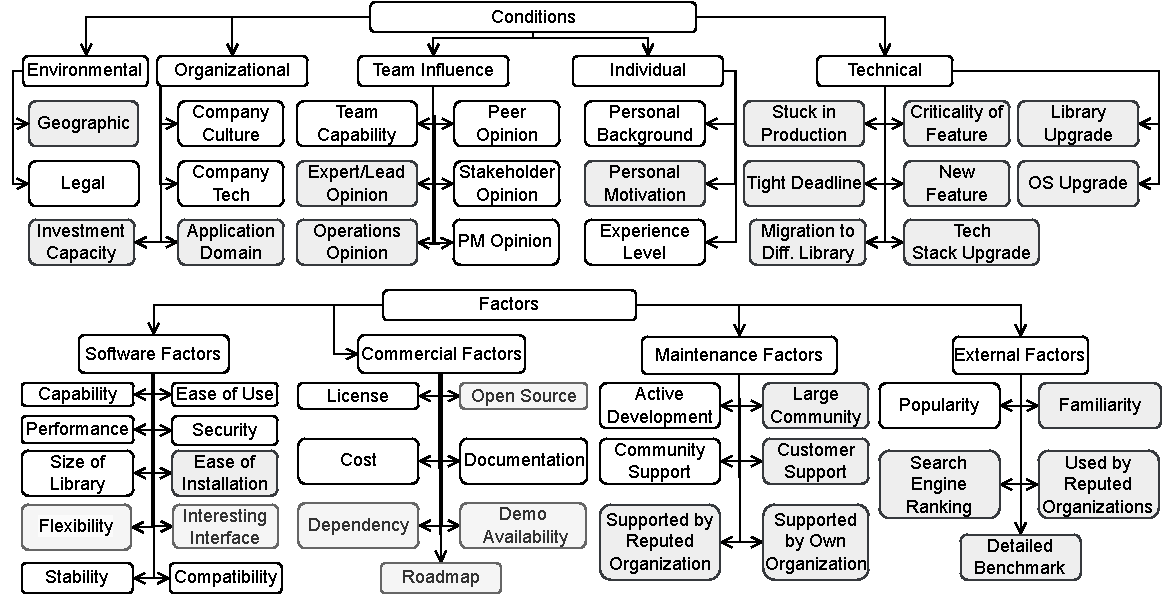
\includegraphics[scale=0.85]{images/conditions.pdf}
%    \caption{Concepts related with factors and conditions %influencing library adoption process}
%    \label{fig:conditions}
%\end{figure*}

\section{Guiding Principles}
In this section, we present the six full patterns associated with the library adoption steps.

\FloatBarrier
\begin{practice}{1}{Just Do It}
\actor{Developers}
\condition{Faster go to market is critical. Developers rewarded for delivering minimum feature on time.}
\concern{How the developers can meet the deadline with relatively less effort?}
\solution{Use a third-party library that reduces the work load and delivery can be done on time}
\consideration{Easy to use, easy to install, popular, and familiar library.}
\steps{Find libraries, compare them, and choose one according to the consideration. Take support from known people or use search engine or Stack Overflow}
\consequence{Can lead to future maintenance burden such as performance bottleneck or security vulnerability.}
\example{For startups, a lot of it [priority] is just speed to market and how much resources is gonna eat up using any specific library.}{P07}
\end{practice}

% \begin{table}[]
%     \centering
%     \caption{Scenario of GP1: Just Do It}
%     \begin{tabular}{p{1cm}p{6.5cm}}
%          \toprule
%             \textbf{GP} & \textbf{Just Do It} \\ 
%             \midrule
%             Actor(s) & Developers \\ 
%             Context & - Faster go to market is critical for business. Developers are often rewarded for delivering minimum viable product on time.
%             - Developers are in their early career and assume higher satisfaction on faster delivery. \\ 
%             Concern & How the developers can meet the deadline in relatively less effort? \\ 
%             Solution & Use a third-party library that reduces the work load and delivery can be done on time \\ 
%             Consider-ation & The library should be easy to use, easy to install, popular, and even better if developer is already familiar with it. \\ 
%             Steps & Find libraries, compare them, and choose one according to the consideration \\ 
%             Support & Take support from known people to know about such library or use search engine, Stack Overflow \\ 
%             Example Trace in Data & For startups, a lot of it [priority] is just speed to market and how much resources is gonna eat up using any specific library. (P07) \\ 
%          \bottomrule
%     \end{tabular}
%     \label{tab:gp1-scenario}
% \end{table}

\begin{practice}{2}{Reuse Robust Component}
\actor{Developers, Senior Developers}
\condition{Mature organization, stable code. Developers concerned of quality, performance \& maintainability.}
\concern{How can the application avoid boiler plate code and follow best design principles?}
\solution{Use a trusted proven third-party library that will keep the code clean and manageable.}
\consideration{Open source, community trusted, stable and high-performing library.}
\steps{Find and compare libraries, review thoroughly by more than one developer. Look into the library's source code repository to analyze the stability, quality of the library, and also consider reputed technical blogs.}
\consequence{Too much analysis and exploration can be an overkill for small features causing delivery delay.}
%\hline
\example{So [this large corporation] as a whole is actually built on the open source libraries that are suitable for our use cases. But that actually has been one of our primary focus as well. If you find a library, use it; only build if you can’t find anything.}{P13}
\end{practice}

% \begin{table}[]
%     \centering
%     \caption{Scenario of GP2: Reuse Robust Component}
%     \begin{tabular}{p{1cm}p{7.5cm}}
%          \toprule
%             \textbf{GP} & \textbf{Reuse Robust Component} \\ 
%             \midrule
%             Actor(s) & Developers, Senior Developers \\ 
%             Context & - Matured organization with stable source code and release pipeline. Application performance and maintainability is a big concern for the team.
%             - Developers with higher experience would be careful about the quality of the application source code. \\ 
%             Concern & How the application can avoid boiler plate code and follow best design principles? \\ 
%             Solution & Use a trusted proven third-party library that will keep the code clean and manageable. \\ 
%             Consider-ation & The library should be open source, trusted by community, stable and provide apppropriate performance metrics required \\ 
%             Steps & Find and compare libraries, review thoroughly by more than one developer. \\ 
%             Support & Look into the library's source code repository to analyze the stability, quality of the library, and also consider reputed technical blogs. \\ 
%             Example Trace in Data & So [this large corporation] as a whole is actually built on the open source libraries that are suitable for our use cases. But that actually has been one of our primary focus as well. If you find a library, use it; only build if you can’t find anything. (P13) \\ 
%          \bottomrule
%     \end{tabular}
%     \label{tab:gp2-scenario}
% \end{table}

%\vspace{-5mm}
\begin{practice}{3}{Maximize Flexibility} % Was Improve Application Structure
\actor{Developers, Architects}
\condition{Large scale software applications have their own structure which evolved over time and may follow some software design principles. System designers want to use new libraries in a way that improves the application structure, or at least does not deteriorate it.}
\concern{How can the architecture be improved or be protected from unwanted rigidity while using a library?}
\solution{Use a library that just fits right with the application in terms of the size and flexibility. Consider wrapping the third-party library in an API to allow replacement of the library without affecting dependent code.}
\consideration{The library should be flexible and should not be too large in size compared to the system.}
\steps{Find, compare, and review libraries. Conduct design review to assess impact on architecture. Review internal organizational content for design principles.}
\example{The moment you have to bring something in because there are new requirements is the time to assess how you've structured your application and does it still serve you and your customers or the business requirements you have. So that’s the opportunity to look at the structural aspect of the application and make sure you do want to avoid changing it or maybe
it's the time to change it.}{P22}
\end{practice}%\vspace{-4mm}

% \begin{table}[h]
%     \centering
%     %\caption{Scenario of GP3: Maximize Flexibility}
%     \begin{tabular}{p{8.5cm}}%{p{1cm}p{7.5cm}}
%          \toprule
%          \textbf{Guiding Principle 3 - Maximize Flexibility} \\% & \textbf{Improve Application Structure} \\ 
%          \midrule
%             \bf{Actor(s).} Developers, Architects \\ %\midrule 
%             \bf{Condition.} Large scale software applications have their own structure which evolved over time and may follow some software design principles. System designers want to use new libraries in a way that improves the application structure, or at least does not deteriorate it.\\ %\midrule 
%             \bf{Concern.} How can the architecture be improved or be protected from unwanted rigidity while using a library?\\ %\midrule 
%             \bf{Solution.} Use a library that just fits right with the application in terms of the size and flexibility. Consider wrapping the third-party library in an API to allow replacement of the library without affecting dependent code.\\ %\midrule 
%             \bf{Consideration}. The library should be flexible and should not be too large in size compared to the system.\\ %\midrule 
%             \bf{Steps.} Find, compare, and review libraries. Conduct design review to assess impact on architecture. Review internal organizational content for design principles.\\ %\midrule 
%             \bf{Example}. \emph{``The moment you have to bring something in because there are new requirements is the time to assess how you've structured your application and does it still serve you and your customers or the business requirements you have. So that’s the opportunity to look at the structural aspect of the application and make sure you do want to avoid changing it or maybe it's the time to change it."}{P22} \\ 

%          \bottomrule
%     \end{tabular}
%     \label{tab:gp3-scenario}
% \end{table}

%\vspace{-5mm}
\begin{practice}{4}{Empower the Team}
\actor{Developers, Tech Leaders}
\condition{Strong company culture to promote transferable skill and provide learning space for developers. 
%Tech leaders may care more for their team's capacity, limitations, and motivations.
The development team may have limitations or strengths in certain technologies. }
\concern{Does the library fit well within the capability of the dev team? Will it provide any transferable skills?}
\solution{Use a library appreciated by the developers}
\consideration{Well documented, popular, easy to use library with customer support.}
\steps{Besides finding a library that fits well with the technology, thoroughly discuss with developers about their opinion and acceptance of the library. Look into official documentation of the library.}
\consequence{May compromise the optimum technology for dev team's limitation. Can keep teams motivated.}
\example{So looking at community popularity helps because then it helps to hire people. It helps to retain people. They like to use technologies that are transferable.}{P19}
\end{practice}%\vspace{-4mm}


% \begin{table}[]
%     \centering
%     \caption{Scenario of GP4: Empower the Team}
%     \begin{tabular}{p{1cm}p{7.5cm}}
%          \toprule
%             \textbf{GP} & \textbf{Empower the Team} \\ 
%             \midrule
%             Actor(s) & Developers, Tech Leaders \\ 
%             Context & - Some organizations may have strong company culture to improve development skill set or for providing comfortable learning space for developers. 
%             - Tech leaders may care more for their team's capacity, limiatation, and motivation.
%             - Development team may have limitation or strength in certain technology  \\ 
%             Concern & Does the library fit well with the capability of the development team? Will it provide them any transferable skill? \\ 
%             Solution & Use a library that is appreciated by the developers \\ 
%             Consider-ation & Library should be well documented, should be community popular so that developers can easily adopt and can refer in future. Also it can have customer support in case developers needs extra help. \\ 
%             Steps & Besides finding a library that fits well with the technology, thoroughly discuss with developers about their opinion and acceptance of the library. \\ 
%             Support & Look into official documentation of the library for documentation and support issues. \\ 
%             Example Trace in Data & So looking at community popularity helps because then you can it helps to hire people. It helps to retain people. They like to use technologies that are transferable (P19) \\ 
%          \bottomrule
%     \end{tabular}
%     \label{tab:gp4-scenario}
% \end{table}

\begin{practice}{5}{Ensure Compliance}
\actor{Developers, Information Security Experts, Legal Experts, Open Source Program Office}
\condition{Because of regulatory compliance or for company culture, some organizations will be more cautious about using third-party libraries for legal, security, and privacy reasons. 
Developers will often have little technical expertise on such specialized issues.
Sometimes small or early stage companies may even ignore the importance of compliance issues.
A few application domains such as health, finance, media are also more regulated and require organizational policies for ensuring compliance.}
\concern{Will there be any penalty or legal complication arising from using a third-party library? How to protect the organization?}
\solution{Use a library which is compliant with the application security standards and legal requirements}
\consideration{The license of the library should be compatible with the business and license of the target software. The security and privacy concerns should be clarified and well taken care of by the library contributors.}
\steps{Reach out to specialists in the organization for taking their expert consent before adopting the library. See the license and security declarations in the library documentation in the source code or package repository.}
\example{We had a very bad experience with this. With the legacy system, we were using so many different libraries and there is a licensing issue and we had to replace half of the library. Otherwise we had to pay lots of money. So that's why we are now very, very concerned about adding any external library, because if we don’t comply with the license, it will be a legal problem.}{P09}
\end{practice}

% \begin{table}[]
%     \centering
%     \caption{Scenario of GP5: Ensure Compliance}
%     \begin{tabular}{p{1cm}p{7.5cm}}
%          \toprule
%             \textbf{GP} & \textbf{Ensure Compliance} \\ 
%             \midrule
%             Actor(s) & Developers, Information Security Experts, Legal Experts, Open Source Program Office \\ 
%             Context & - Because of regulatory compliance or for company culture, some organizations will be more cautious about using third-party libraries for legal, security, and privacy reasons. 
%             - Developers will often have little technical expertise on such speialized issues
%             - Sometimes small or early stage companies may even ignore the importance of compliance issues
%             - Few application domains such as health, finance, media are also more regulated and require organizational policies for ensuring compliance. \\ 
%             Concern & Will there be any penalty or legal complication arising from using a third-party library? How to protect the organization? \\ 
%             Solution & Use a library which is compliant with the application security standards and legal requirements \\ 
%             Consider-ation & License of the library should be compatible with the business and license of the target software. The security and privacy concerns should be clarified and well take care of by the library contributors. \\ 
%             Steps & Reach out to specialists in the organization for taking their expert consent before adopting the library. \\ 
%             Support & See the license and security declarations in the library documentation in the source code or package repository. \\ 
%             Example Trace in Data & we had a very bad experience with this. With the legacy system, we were using so many different libraries and there is a licensing issue and we had to replace half of the library. Otherwise we had to pay lots of money. So that’s why we are now very, very concerned about adding any external library, because if we don’t comply with the license, it will be a legal problem. (P09) \\ 
%          \bottomrule
%     \end{tabular}
%     \label{tab:gp5-scenario}
% \end{table}

\begin{practice}{6}{Maintain Continuous Stability}
\actor{Developers, DevOps}
\condition{Some software applications are developed and maintained for long term. A third-party library used in such a product can have bugs or vulnerabilities that need to be fixed. Sometimes, the contributors of the library may not continue to fix bugs or improve with new features. Sometimes libraries may not have backwards compatibility and when developers upgrade, their existing system can break.}
\concern{How will developers ensure that a library is well maintained in foreseeable future and that they can keep using the library without breaking their application?}
\solution{Use a library with good history of maintenance and prepare to continuously upgrade the library in future}
\consideration{Selected libraries should be actively maintained by contributors, supported by reputed organizations, and have larger community.}
\steps{Analyze the maintenance and issue history of the library to assess the active development practices or the library. Establish a process for software bill of materials to document all third-party library dependencies and their upgrade plan in conjunction with DevOps teams. Look into source code commit and issue history from source repository and download usage trend from package repository.}
\example{When we integrated the updated version our whole interface broke. And we had to change a lot of code, all the interceptors, interfaces, everything\ldots This maintenance is quite hard. It's actually a full time work to always keep updated, to always stay updated.}{P14}
\end{practice}

% \begin{table}[]
%     \centering
%     \caption{Scenario of GP6: Maintain Continuous Stability}
%     \begin{tabular}{p{1cm}p{7.5cm}}
%          \toprule
%             \textbf{GP} & \textbf{Maintain Continuous Stability} \\
%             \midrule
%             Actor(s) & Developers, DevOps \\ 
%             Context & - Some software applications are developed and maintained for long term. A third-party library used in such a product can have bugs or vulnerabilities that need to be fixed. Sometimes, the contributors of the library may not continue to fix bugs or improve with new features. Sometimes libraries may not have backwards compatibility and when developers upgrade, their existing system can break. \\ 
%             Concern & How developers will ensure that a library is well maintained in foreseeable future and can keep using the library without breaking their application? \\ 
%             Solution & Use a library with good history of maintenance and prepare to continuously upgrade the library in future \\ 
%             Consider-ation & Selected libraries should be actively maintained by contributors, supported by reputed organizations, and have larger community. \\ 
%             Steps & Analyze the maintenance and issue history of the library to assess the active development practices or the library. Establish a process for software bill of materials to document all third-party library dependencies and their upgrade plan in conjunction with DevOps teams. \\ 
%             Support & Look into source code commit and issue history from source repository and download usage trend from package repository. \\ 
%             Example Trace in Data & when we integrated the updated version our whole interface broke. And we had to change a lot of code, all the interceptors, interfaces, everything... This maintenance is quite hard. It’s actually a full time work to always keep updated, to always stay updated. (P14) \\ 
%          \bottomrule
%     \end{tabular}
%     \label{tab:gp6-scenario}
% \end{table}


\end{document}
